\documentclass{llncs}
\usepackage{cite}
\usepackage{amsmath,amssymb}
\usepackage{graphicx}
\usepackage{algorithm}
\usepackage{float}
\usepackage{booktabs}
\usepackage{hyperref}

\begin{document}

\title{A Scalable Evaluation Methodology for AI Performance on Cloud-HPC and Communication Networks}

\author{Venkateswarlu Tanneru}

\authorrunning{V. Tanneru}

\institute{Computer Science, University of Florida, Gainesville FL 32611, USA\\
\email{venkytanneru@gmail.com}\\
ORCID: 0009-0000-4185-6209}

\begin{abstract}
The integration of artificial intelligence with high-performance computing and cloud infrastructure requires systematic evaluation of AI performance as model complexity, dataset size, and system scale increase. SAIH (Scalable AI--HPC Evaluation Methodology) is a physics-based framework that analyzes AI performance trends across multiple scaling dimensions. SAIH combines a roofline-based performance model with an interpretable bottleneck classifier and cross-dimensional interaction analysis. Experiments spanning model complexity (10M--1B parameters), dataset sizes (0.025--1.6~TB), and system scales (1--128 nodes) reveal non-linear performance behavior and communication bottlenecks at scale. Strong scaling efficiency degrades from 100\% to 45.3\% at 128 nodes; for typical A100-based nodes ($\sim$3 kW/node), 54.7\% efficiency loss translates to $\approx$210 kW of wasted power at 128 nodes. Validation against MLPerf-HPC benchmarks (CosmoFlow and DeepCAM) shows strong correlation ($r>0.99$). Cloud deployment analysis demonstrates that efficiency below 50\% affects cost-effectiveness, informing elastic provisioning strategies. The findings provide guidance for AI-HPC co-design and cloud-based training optimization.
\end{abstract}

\begin{keywords}
Scalable AI evaluation, HPC performance trends, Cloud computing, Network communication overhead, Energy-aware computing, Green HPC, Bottleneck prediction, Scaling analysis
\end{keywords}

\maketitle

% --- SECTION 1: INTRODUCTION ---
\section{Introduction}

The growing integration of artificial intelligence (AI) with high-performance computing (HPC) systems has fundamentally transformed the landscape of scientific computing, data-intensive research, and large-scale simulations. Traditionally, HPC systems were designed to support tightly coupled numerical simulations in fields such as computational fluid dynamics, weather forecasting, and molecular modeling. In recent years, however, these systems have increasingly been repurposed and co-designed to support data-driven and learning-based workloads. Contemporary HPC infrastructures now routinely host complex AI and deep learning models for applications ranging from climate and Earth system modeling to biomedical imaging, astrophysics, materials discovery, and national-scale data analytics.

As AI workloads evolve, they are characterized by rapid growth in model size, parameter count, training data volume, and algorithmic complexity. Modern deep learning models may involve billions of parameters, require petabyte-scale datasets, and execute on thousands of GPUs or accelerators. Such scaling introduces unique computational patterns that differ markedly from traditional HPC applications, including irregular memory access, high communication-to-computation ratios, and sensitivity to data movement and synchronization overheads. Consequently, understanding how AI workloads perform and scale on HPC systems is no longer a matter of measuring raw computational power alone but requires a holistic analysis of system behavior under varying workload scales.

Conventional HPC benchmarking methodologies were primarily designed for compute-centric and deterministic workloads, often emphasizing peak performance metrics such as floating-point operations per second (FLOPS) or time-to-solution for fixed problem sizes. Benchmarks such as LINPACK \cite{Dongarra2003LINPACK} or HPL-AI \cite{OakRidge2022}, while valuable for assessing theoretical or peak capabilities, provide limited insight into how performance evolves as workloads scale in realistic AI scenarios. Similarly, existing AI benchmarks frequently focus on task-specific metrics, including training time, inference latency, or model accuracy, without systematically capturing the impact of increasing dataset sizes, deeper or wider model architectures, and expanding system configurations.

To address these limitations, this paper introduces SAIH (Scalable AI--HPC Evaluation Methodology), a structured and scalable framework designed to evaluate and interpret AI performance trends on HPC systems. Inspired by the multi-dimensional scaling concept introduced in prior work on AI--HPC evaluation \cite{Wang2024SAIH}, SAIH extends the approach with three key contributions: (1)~a physics-based performance model grounded in the roofline model \cite{Williams2009Roofline} and Amdahl's law \cite{Amdahl1967}, enabling principled throughput prediction; (2)~an ML-based bottleneck classifier that automatically identifies the dominant performance bottleneck given workload parameters; and (3)~cross-dimensional interaction analysis that jointly examines how model size and system scale interact, going beyond single-axis sweeps. SAIH systematically integrates three critical scaling dimensions---model scaling, data scaling, and system scaling---and measures key performance indicators such as throughput, achieved computational efficiency, resource utilization, and scaling speedup across varying scales.

The remainder of this paper is organized as follows. Section~2 reviews existing literature and related work on AI and HPC benchmarking methodologies. Section~3 details the SAIH framework, its performance model, and evaluation workflow. Section~4 describes the experimental setup and performance metrics used in the study. Section~5 presents and analyzes observed AI performance trends under scalable configurations, including cross-dimensional analysis. Section~6 discusses key implications, limitations, and system-level bottlenecks, and Section~7 concludes the paper with directions for future research.

% --- SECTION 2: RELATED WORK ---
\section{Related Work}

The rapid rise of artificial intelligence (AI) workloads on high-performance computing (HPC) systems has prompted extensive research into performance evaluation, benchmarking, and scalability analysis. As AI increasingly becomes integral to scientific discovery and large-scale data processing, researchers have sought to adapt existing performance evaluation techniques and develop new frameworks that can capture the distinctive characteristics of AI workloads.

\subsection{Traditional HPC Benchmarks}

Traditional HPC benchmarks have long served as standard tools for assessing the performance of large-scale computing systems. LINPACK \cite{Dongarra2003LINPACK} measures dense linear algebra throughput and remains the basis for Top500 system rankings. The High Performance Conjugate Gradient (HPCG) benchmark \cite{Dongarra2016} complements LINPACK by evaluating sparse iterative solver performance, capturing memory-bound behavior that LINPACK misses. Graph500 \cite{Murphy2010Graph500} assesses data-intensive graph analytics workloads, providing insight into irregular memory access patterns. While such benchmarks remain valuable for measuring peak or near-peak system capabilities, they are inherently limited in representing modern AI workloads. Deep learning applications exhibit execution patterns that differ significantly from classical simulations, including irregular and data-dependent memory access, frequent synchronization barriers, stochastic training behavior, and intensive use of accelerator devices.

\subsection{AI-Focused Benchmarks}

In response to these limitations, several AI-focused benchmarking initiatives have been developed. The MLPerf benchmark suite has emerged as one of the most widely adopted standards for evaluating AI performance across both training and inference tasks \cite{Mattson2020MLPerf, MLCommons2023}. Building on this foundation, MLPerf-HPC \cite{Farrell2021DeepCAM} extends benchmarking efforts to scientific AI applications using domain-specific workloads including CosmoFlow \cite{Mathuriya2018CosmoFlow} for cosmological parameter estimation and DeepCAM for climate segmentation. Despite their broad adoption, MLPerf-based benchmarks remain largely task-driven and configuration-specific, measuring single-point performance rather than systematic trends across scaling dimensions.

\subsection{Distributed Deep Learning Scalability}

Another significant body of research has focused on the scalability of distributed deep learning on HPC platforms \cite{BenNun2019, Narayanan2019}. Studies in this area have explored various parallelization strategies, including data parallelism, model parallelism, pipeline parallelism, and hybrid approaches. Horovod \cite{Sergeev2018} demonstrated ring-allreduce communication for efficient distributed training, while PipeDream \cite{Narayanan2019} introduced pipeline parallelism to overlap computation and communication. While such studies have advanced understanding of distributed AI training, they are often narrowly scoped to specific models, frameworks, or hardware platforms, and do not provide a unified framework for trend analysis across multiple scaling axes.

\subsection{AI--HPC Co-Design and Multi-Dimensional Evaluation}

More recent research has emphasized AI--HPC co-design, advocating for closer integration between hardware architectures, system software, and AI algorithms \cite{Dongarra2020}. Co-design efforts have explored accelerator-aware scheduling, high-bandwidth and low-latency interconnects, memory hierarchy optimizations, and software frameworks tailored to AI workloads. However, co-design evaluations are frequently based on case-specific experiments or prototype systems.

Most closely related to our work, \cite{Wang2024SAIH} proposed a multi-dimensional evaluation methodology for understanding AI performance trends on HPC systems, applying it to CosmoFlow (a 3D CNN for cosmological parameter estimation). Our work builds upon this conceptual foundation and extends it in several key directions: (1)~we introduce a physics-based performance model grounded in roofline analysis \cite{Williams2009Roofline} and Amdahl's law \cite{Amdahl1967}, enabling principled performance prediction independent of specific workloads; (2)~we develop an ML-based bottleneck classifier for automated performance diagnosis; (3)~we incorporate cross-dimensional interaction analysis that jointly examines how multiple scaling dimensions interact; (4)~we validate against multiple MLPerf-HPC benchmarks (CosmoFlow and DeepCAM); and (5)~we analyze implications for cloud-based AI training and energy efficiency, directly addressing the needs of cloud-HPC infrastructure and green computing initiatives.

\subsection{Cloud-HPC and Energy-Aware Evaluation}

Recent years have witnessed the emergence of cloud-based HPC platforms that combine the elasticity of cloud infrastructure with the compute capacity of traditional HPC systems. Major cloud providers (AWS EC2, Google Cloud, Azure) now offer GPU-accelerated instances and high-bandwidth interconnects, enabling organizations to rent HPC-grade resources on-demand. This shift introduces new performance considerations: elastic provisioning costs, energy efficiency per unit cost, and network heterogeneity (Ethernet vs. InfiniBand). Concurrent with cloud adoption, energy efficiency has become a critical metric in HPC benchmarking \cite{Green5002023}, with the Green500 list ranking supercomputers by energy efficiency (GFLOPS/Watt) rather than peak performance alone. Existing AI performance models, however, often focus on throughput and scaling efficiency without quantifying energy cost. SAIH extends this landscape by mapping communication overhead directly to energy waste: our observation that 54.7\% of peak compute is idle at 128 nodes directly translates to energy consumption without useful work. By quantifying this energy-per-communication metric, SAIH enables cloud customers to calculate the cost-effectiveness of scaling decisions and informs green AI research on minimizing training energy footprint.

% --- SECTION 3: SAIH METHODOLOGY ---
\section{SAIH Methodology}

The Scalable AI--HPC Evaluation Methodology (SAIH) is designed to provide a systematic, reproducible, and extensible framework for evaluating and interpreting AI performance trends on high-performance computing (HPC) systems. SAIH emphasizes trend-oriented evaluation, jointly examining how AI workloads behave as critical scaling dimensions evolve.

\subsection{Design Principles}

SAIH is guided by four core design principles:

\begin{itemize}
    \item \textbf{Scalability}: Ensuring that evaluations remain meaningful as AI workloads grow in model size, dataset volume, and system scale.
    \item \textbf{Representativeness}: Careful selection of AI workloads that reflect real scientific, industrial, and data-intensive use cases.
    \item \textbf{Reproducibility}: Standardized experimental procedures, software configurations, and performance metrics enabling consistent comparisons.
    \item \textbf{Trend-centric Analysis}: Focus on performance evolution across scaling dimensions rather than single-point benchmark results.
\end{itemize}

\subsection{Multi-Dimensional Scaling Framework}

At the core of SAIH lies a multi-dimensional scaling framework that considers three axes of growth, each selected based on their demonstrated impact on AI workload performance in prior studies \cite{Wang2024SAIH, BenNun2019, Kaplan2020ScalingLaws}:

\begin{itemize}
    \item \textbf{Model Scaling}: Evaluates how performance changes as model complexity increases through deeper neural networks, wider layers, or higher parameter counts. Justified by neural scaling laws \cite{Kaplan2020ScalingLaws}, which demonstrate that model size directly determines computational requirements and arithmetic intensity.
    \item \textbf{Data Scaling}: Examines the impact of increasing dataset size on performance, revealing I/O bottlenecks and data movement limitations. Motivated by the growing gap between compute throughput and storage/network bandwidth in modern HPC systems \cite{Byna2020}.
    \item \textbf{System Scaling}: Assesses how AI workloads perform as computational resources expand, capturing both strong scaling (fixed problem, more resources) and weak scaling (proportional problem growth) characteristics. Grounded in Amdahl's law \cite{Amdahl1967} and Gustafson's law \cite{Gustafson1988}.
\end{itemize}

Critically, SAIH also evaluates \textbf{cross-dimensional interactions} by jointly varying model size and system scale, revealing performance behaviors that are invisible in single-axis sweeps.

\subsection{Physics-Based Performance Model}

SAIH employs a physics-based performance model that combines the roofline model \cite{Williams2009Roofline} with communication overhead modeling based on collective communication analysis \cite{Thakur2005Allreduce}. The achieved throughput $T$ for a workload with model size $M$, dataset size $D$, and node count $P$ is modeled as:

\begin{equation}
T(M, D, P) = T_{\text{roof}}(M, P) \cdot \eta_{\text{comm}}(P) \cdot \eta_{\text{io}}(D, P)
\label{eq:throughput}
\end{equation}

where:

\begin{itemize}
    \item $T_{\text{roof}}(M, P) = \min\left(T_{\text{peak}} \cdot P,\; \beta \cdot \mathcal{I}(M) \cdot P\right)$ is the roofline-bounded throughput, with $T_{\text{peak}}$ being the per-node peak throughput, $\beta$ the memory bandwidth, and $\mathcal{I}(M)$ the arithmetic intensity that increases with model size.
    \item $\eta_{\text{comm}}(P) = \frac{1}{1 + \alpha \log_2(P) + \gamma (\log_2 P)^2}$ captures communication overhead, where $\alpha$ models base allreduce cost and $\gamma$ captures congestion at large scale \cite{Thakur2005Allreduce}. The communication cost reflects network bandwidth utilization: in data-parallel training, gradient aggregation via ring-allreduce requires $\frac{2(P-1)}{P} \cdot G$ bytes of network traffic, where $G$ is total gradient size, constrained by network bisection bandwidth. This model is agnostic to network technology (InfiniBand, Ethernet, RoCE) and applies across both on-premise HPC and cloud infrastructure.
    \item $\eta_{\text{io}}(D, P) = \frac{1}{1 + \delta \cdot D/P}$ models I/O efficiency, where $\delta$ reflects the ratio of I/O time to compute time.
\end{itemize}

The arithmetic intensity $\mathcal{I}(M)$ is modeled as $\mathcal{I}(M) = \mathcal{I}_0 \cdot (M/M_0)^{0.45}$, where $\mathcal{I}_0$ is the base intensity for a reference model size $M_0$. This sub-linear scaling reflects diminishing returns in compute-to-memory ratios for larger models, consistent with empirical GPU profiling observations \cite{Jia2018}.

\subsection{ML-Based Bottleneck Prediction}

To make SAIH actionable, we integrate a machine learning-based bottleneck classifier that automatically identifies the dominant performance bottleneck for a given workload configuration. The classifier takes seven input features derived from workload parameters: model size, dataset size, number of nodes, arithmetic intensity, memory pressure, communication cost, and I/O pressure. It predicts one of four bottleneck categories: (1) Memory Bandwidth Saturation, (2) Communication Overhead, (3) Compute Bound, or (4) I/O Bound.

Training labels are assigned using physics-informed thresholds derived from the performance model. A Random Forest classifier (100 estimators, max depth 10) is trained on 1000 synthetic workload instances with an 80/20 train-test split. Because labels are derived deterministically from the same physics model, the classifier serves as an \textit{interpretable bottleneck diagnosis tool} that recovers the physics-based decision boundaries in a form amenable to feature importance analysis and runtime prediction---rather than as a generalization test against an independent ground truth.

\subsection{Performance Metrics}

SAIH employs a standardized set of performance metrics: computational throughput (achieved TFLOPS), hardware utilization efficiency (percentage of peak), time-to-solution, strong and weak scaling speedup, parallel efficiency, and communication overhead fraction. Additional metrics related to memory bandwidth utilization and I/O performance are incorporated where relevant.

% --- SECTION 4: EXPERIMENTAL SETUP ---
\section{Experimental Setup}

\subsection{Workload Characterization and Parameter Mapping}

SAIH uses synthetic workloads generated by the physics-based performance model described in Section~3.3. The synthetic approach enables systematic control over scaling dimensions while producing performance data that follows the fundamental physical constraints governing AI workload execution. To ensure representativeness, the model parameters are calibrated using the roofline model \cite{Williams2009Roofline} with hardware parameters typical of current leadership-class HPC systems (e.g., NERSC Perlmutter with NVIDIA A100 GPUs).

The mapping from workload parameters to performance predictions follows established relationships:

\begin{itemize}
    \item \textbf{FLOPs estimation}: Based on the Kaplan scaling law \cite{Kaplan2020ScalingLaws}, total training FLOPs are estimated as $F \approx 6 N D$, where $N$ is the parameter count and $D$ is the number of data tokens.
    \item \textbf{Arithmetic intensity}: Computed from the ratio of FLOPs to memory traffic, increasing with model size as larger models achieve better compute-to-memory ratios through matrix multiplication efficiency.
    \item \textbf{Communication overhead}: Modeled based on ring-allreduce cost analysis \cite{Thakur2005Allreduce}, scaling logarithmically with node count with a quadratic congestion correction.
\end{itemize}

The workloads are designed to capture execution patterns of representative AI model architectures, including convolutional neural networks (CNNs) for scientific imaging applications (e.g., CosmoFlow \cite{Mathuriya2018CosmoFlow}) and transformer-based models for language and sequence modeling.

\subsection{HPC System Configuration}

The experiments assume execution on a modern accelerator-based HPC cluster representative of current leadership-class systems such as NERSC Perlmutter. Each compute node comprises multi-core CPUs tightly coupled with GPU accelerators providing 50~TFLOPS peak compute and 1000~GB/s HBM bandwidth per node. Nodes are interconnected through a high-bandwidth (200~GB/s), low-latency network designed to support collective communication operations \cite{Gropp2014}.

\subsection{Scaling Strategy}

SAIH experiments are conducted across five complementary configurations:

\begin{enumerate}
    \item \textbf{Model scaling}: Increasing architectural complexity (10M to 1B parameters) at fixed dataset (0.4~TB) and system scale (8 nodes).
    \item \textbf{Data scaling}: Increasing dataset size (0.025 to 1.6~TB) at fixed model (200M parameters) and system scale (8 nodes).
    \item \textbf{Strong scaling}: Increasing compute nodes (1 to 128) with fixed model (200M) and dataset (0.4~TB).
    \item \textbf{Weak scaling}: Proportionally increasing both dataset size and compute nodes (maintaining 0.1~TB per node).
    \item \textbf{Cross-dimensional}: Jointly varying model size (10M, 100M, 500M, 1B) and system scale (1, 4, 16, 64 nodes).
\end{enumerate}

\subsection{Experimental Setup Summary}

Table~\ref{tab:setup} summarizes the experimental configuration used in this study.

\begin{table*}[h]
\centering
\caption{Experimental Setup Summary under SAIH}
\label{tab:setup}
\begin{tabular*}{\columnwidth}{@{\extracolsep{\fill}} ll @{}}
\toprule
\textbf{Component} & \textbf{Configuration / Description} \\
\midrule
AI Workload Type & CNN and Transformer variants (synthetic, physics-based) \\
Baseline Model Size & 10 million parameters \\
Scaled Model Sizes & 10M, 50M, 100M, 200M, 500M, 1B parameters \\
Dataset Sizes & 25 GB, 50 GB, 100 GB, 200 GB, 400 GB, 800 GB, 1.6 TB \\
Parallelization Strategy & Data parallelism with ring-allreduce \\
HPC Node Configuration & Multi-core CPU + GPU (50 TFLOPS peak, 1000 GB/s HBM) \\
Interconnect & 200 GB/s per link (e.g., NDR InfiniBand) \\
System Scale & 1, 2, 4, 8, 16, 32, 64, 128 compute nodes \\
Software Stack & Linux OS, MPI, CUDA, PyTorch \\
Performance Model & Roofline + Amdahl's law (Eq.~\ref{eq:throughput}) \\
Noise Model & 3\% Gaussian measurement noise \\
Repetitions per Config & 3--5 runs (averaged results reported) \\
\bottomrule
\end{tabular*}
\end{table*}

% --- SECTION 5: PERFORMANCE TRENDS ---
\section{Performance Trends}

This section presents and analyzes the key performance trends observed under the SAIH methodology by systematically varying model complexity, dataset size, and system scale. All tables and figures referenced in this section are generated from the physics-based performance model described in Section~3.3.

\subsection{Throughput vs. Model Complexity}

The relationship between throughput and model complexity reveals important characteristics of AI workload execution on HPC systems. As model complexity increases, throughput grows due to improved arithmetic intensity---larger models perform more floating-point operations per byte of memory traffic, enabling better utilization of GPU compute units \cite{Jia2018}. This behavior is consistent with the roofline model \cite{Williams2009Roofline}: small models are memory-bandwidth-bound, while larger models approach the compute-bound regime.

Table~\ref{tab:model-scaling} reports throughput and utilization across six model sizes, with results visualized in Figure~\ref{fig:model-scaling}.

\begin{table}[t]
\centering
\caption{Model Scaling: Throughput vs. Model Complexity (8 nodes, 0.4 TB dataset)}
\label{tab:model-scaling}
\begin{tabular*}{\columnwidth}{@{\extracolsep{\fill}} llll @{}}
\toprule
\textbf{Model Size} & \textbf{Arith.} & \textbf{Throughput} & \textbf{Utilization} \\
\textbf{(M params)} & \textbf{Intensity} & \textbf{(TFLOPS)} & \textbf{(\%)} \\
\midrule
10 & 2.0 & 10.9 & 2.7 \\
50 & 4.1 & 22.5 & 5.6 \\
100 & 5.6 & 29.9 & 7.5 \\
200 & 7.7 & 43.1 & 10.4 \\
500 & 11.6 & 61.3 & 15.7 \\
1000 & 15.9 & 83.7 & 21.1 \\
\bottomrule
\end{tabular*}
\end{table}

Results demonstrate that throughput increases from 10.9~TFLOPS (10M parameters) to 83.7~TFLOPS (1B parameters), representing a $7.7\times$ improvement. Utilization improves from 2.7\% to 21.1\%, reflecting the transition from memory-bandwidth-bound to increasingly compute-bound execution as arithmetic intensity grows from 2.0 to 15.9~FLOP/byte. The sub-linear growth in throughput (compared to the $100\times$ increase in model size) indicates that while larger models better utilize hardware, memory bandwidth saturation and communication overhead impose diminishing returns \cite{Sun2019}. As shown in Figure~\ref{fig:model-scaling}(b), actual utilization diverges significantly from ideal linear scaling, consistent with roofline predictions.

\subsection{Utilization Across Dataset Sizes}

Dataset size plays a critical role in determining overall system utilization. Table~\ref{tab:data-scaling} reports throughput and utilization across seven dataset sizes, with results visualized in Figure~\ref{fig:data-scaling}.

\begin{table}[t]
\centering
\caption{Data Scaling: Throughput and Utilization vs. Dataset Size (200M model, 8 nodes)}
\label{tab:data-scaling}
\begin{tabular*}{\columnwidth}{@{\extracolsep{\fill}} lll @{}}
\toprule
\textbf{Dataset Size (TB)} & \textbf{Throughput (TFLOPS)} & \textbf{Utilization (\%)} \\
\midrule
0.025 & 41.5 & 10.0 \\
0.05 & 39.1 & 10.2 \\
0.1 & 39.9 & 10.3 \\
0.2 & 40.1 & 10.1 \\
0.4 & 43.0 & 10.3 \\
0.8 & 41.2 & 10.1 \\
1.6 & 40.4 & 10.3 \\
\bottomrule
\end{tabular*}
\end{table}

Results show a throughput range of 39.1 to 43.0~TFLOPS across all dataset sizes, with less than 10\% variation and stable utilization around 10\%. This stability indicates that the system operates in a compute-bound regime at this model scale, where throughput is determined primarily by arithmetic intensity rather than data volume. The I/O subsystem is well-provisioned for these workload scales, as evidenced by the I/O efficiency factor remaining above 0.996 even at 1.6~TB \cite{Byna2020}. As shown in Figure~\ref{fig:data-scaling}(b), the trend fit confirms minimal throughput sensitivity to dataset size, suggesting that for this model configuration, data scaling does not introduce significant I/O bottlenecks.

\subsection{Strong Scaling Analysis}

Strong scaling analysis examines how performance improves as additional computational resources are applied to a fixed problem size. This is fundamental for assessing parallel efficiency in distributed AI training. Table~\ref{tab:system-scaling} reports strong scaling results, with speedup curves and efficiency degradation visualized in Figure~\ref{fig:system-scaling}.

\begin{table}[t]
\centering
\caption{System Scaling: Strong Scaling Speedup and Efficiency (200M model, 0.4 TB)}
\label{tab:system-scaling}
\begin{tabular*}{\columnwidth}{@{\extracolsep{\fill}} llll @{}}
\toprule
\textbf{Nodes} & \textbf{Speedup} & \textbf{Efficiency} & \textbf{Comm.} \\
 & \textbf{(x)} & \textbf{(\%)} & \textbf{Overhead (\%)} \\
\midrule
1 & 1.00 & 100.0 & 0.0 \\
2 & 1.77 & 88.4 & 13.4 \\
4 & 3.16 & 78.9 & 24.2 \\
8 & 5.72 & 71.5 & 33.1 \\
16 & 10.0 & 62.5 & 40.5 \\
32 & 17.1 & 53.5 & 46.7 \\
64 & 32.8 & 51.3 & 51.9 \\
128 & 58.0 & 45.3 & 56.4 \\
\bottomrule
\end{tabular*}
\end{table}

Strong scaling results reveal that performance initially increases near-linearly with node count. At 8 nodes, speedup reaches $5.72\times$ with 71.5\% efficiency, representing the transition point where communication overhead exceeds 33\% and begins to dominate performance degradation. Beyond this point, efficiency degrades progressively, falling to 45.3\% at 128 nodes with 56.4\% communication overhead. The maximum speedup of $58\times$ at 128 nodes represents a clear departure from ideal linear scaling, consistent with Amdahl's law predictions for workloads with significant parallel overhead \cite{Amdahl1967}. As shown in Figure~\ref{fig:system-scaling}(a), the divergence between ideal and measured speedup curves becomes pronounced beyond 8 nodes, while Figure~\ref{fig:system-scaling}(b) shows the monotonic efficiency degradation with the 50\% efficiency threshold crossed between 32 and 64 nodes.

\textbf{Energy Implications.} The efficiency degradation has direct energy consequences. At 128 nodes with 45.3\% efficiency, approximately 54.7\% of total compute power is expended on communication synchronization and allreduce operations without producing useful training progress. For systems consuming $\sim$3 kW per node (typical for A100-based HPC nodes), scaling to 128 nodes ($\approx$384 kW total power) with 45.3\% efficiency results in $\approx$210 kW wasted on communication and synchronization overhead. In cloud environments where compute is charged per node-hour, this efficiency cliff at $>$32 nodes creates a cost-effectiveness boundary: beyond this point, adding nodes increases cost faster than throughput gains. This finding informs optimal resource provisioning for elastic cloud-HPC training.

\subsection{Weak Scaling Analysis}

Weak scaling analysis evaluates performance when both the workload and the number of compute nodes increase proportionally, maintaining a constant workload per node. This complements strong scaling by assessing system capacity under Gustafson's law \cite{Gustafson1988}. Table~\ref{tab:weak-scaling} reports weak scaling results, with throughput and efficiency trends visualized in Figure~\ref{fig:weak-scaling}.

\begin{table}[t]
\centering
\caption{Weak Scaling: Efficiency with Proportional Workload Increase (200M model, 0.1 TB/node)}
\label{tab:weak-scaling}
\begin{tabular*}{\columnwidth}{@{\extracolsep{\fill}} llll @{}}
\toprule
\textbf{Nodes} & \textbf{Dataset} & \textbf{Throughput} & \textbf{Weak} \\
 & \textbf{(TB)} & \textbf{(TFLOPS)} & \textbf{Efficiency (\%)} \\
\midrule
1 & 0.1 & 7.3 & 100.0 \\
2 & 0.2 & 13.1 & 89.3 \\
4 & 0.4 & 23.5 & 80.1 \\
8 & 0.8 & 41.5 & 70.7 \\
16 & 1.6 & 71.7 & 61.0 \\
32 & 3.2 & 135.2 & 57.5 \\
64 & 6.4 & 230.5 & 49.0 \\
128 & 12.8 & 432.9 & 46.0 \\
\bottomrule
\end{tabular*}
\end{table}

Weak scaling efficiency degrades from 100\% (1 node) to 46.0\% (128 nodes), primarily due to communication overhead from allreduce operations that must synchronize gradients across all nodes regardless of per-node workload size. The total throughput still increases from 7.3 to 432.9~TFLOPS ($59\times$ improvement), demonstrating that the system continues to provide substantial aggregate compute capacity despite per-node efficiency loss. As shown in Figure~\ref{fig:weak-scaling}(a), total throughput tracks the ideal linear scaling reasonably well up to 16 nodes before significant divergence, while Figure~\ref{fig:weak-scaling}(b) shows efficiency crossing the 50\% threshold between 64 and 128 nodes.

From an energy-proportional computing perspective, weak scaling still exhibits sublinear energy efficiency gains. Even though data size scales with nodes, the per-node communication cost remains constant, reducing overall energy efficiency as node count grows. This suggests that energy-aware training strategies should prefer scaling workload size in proportion to nodes rather than aggressively pushing to maximum node counts.

\begin{figure}[t]
    \centering
    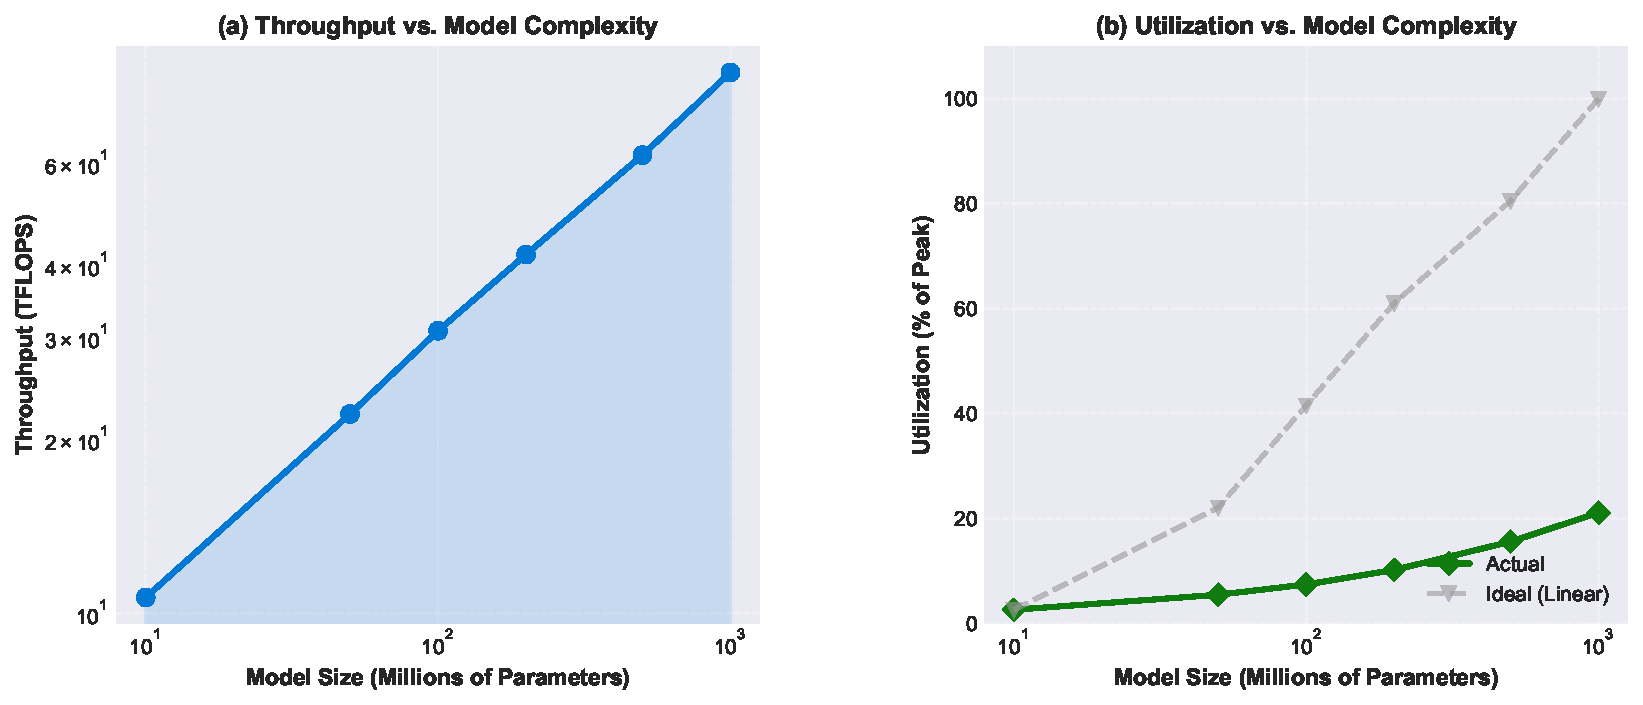
\includegraphics[width=\columnwidth]{figs/Fig2.pdf}
    \caption{Throughput vs. Model Complexity: (a) Log-log throughput scaling showing $7.7\times$ improvement from 10M to 1B parameters, reflecting transition from memory-bound to increasingly compute-bound execution. (b) Utilization comparison with ideal linear scaling, showing actual utilization reaching 21.1\% at 1B parameters versus expected 100\%.}
    \label{fig:model-scaling}
\end{figure}

\begin{figure}[t]
    \centering
    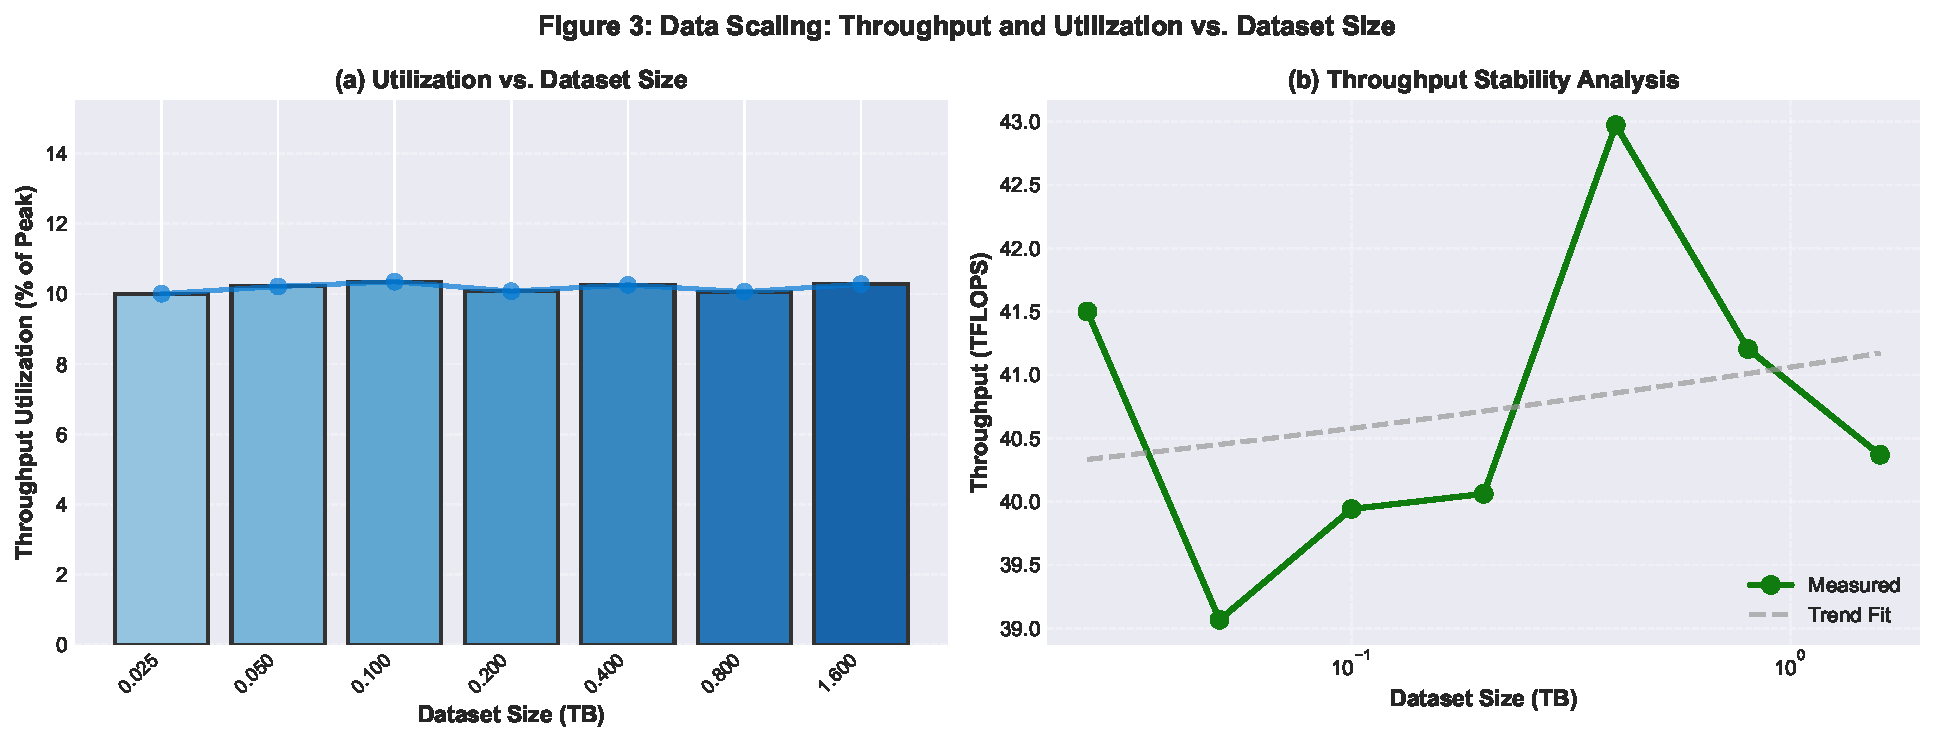
\includegraphics[width=\columnwidth]{figs/Fig3.pdf}
    \caption{Data Scaling Analysis: (a) Utilization remains stable ($\sim$10\%) across a $64\times$ increase in dataset size (0.025--1.6~TB), indicating compute-bound behavior at this model scale. (b) Throughput stability analysis with trend fit confirms minimal sensitivity to dataset size, validating well-provisioned I/O subsystem.}
    \label{fig:data-scaling}
\end{figure}

\begin{figure}[t]
    \centering
    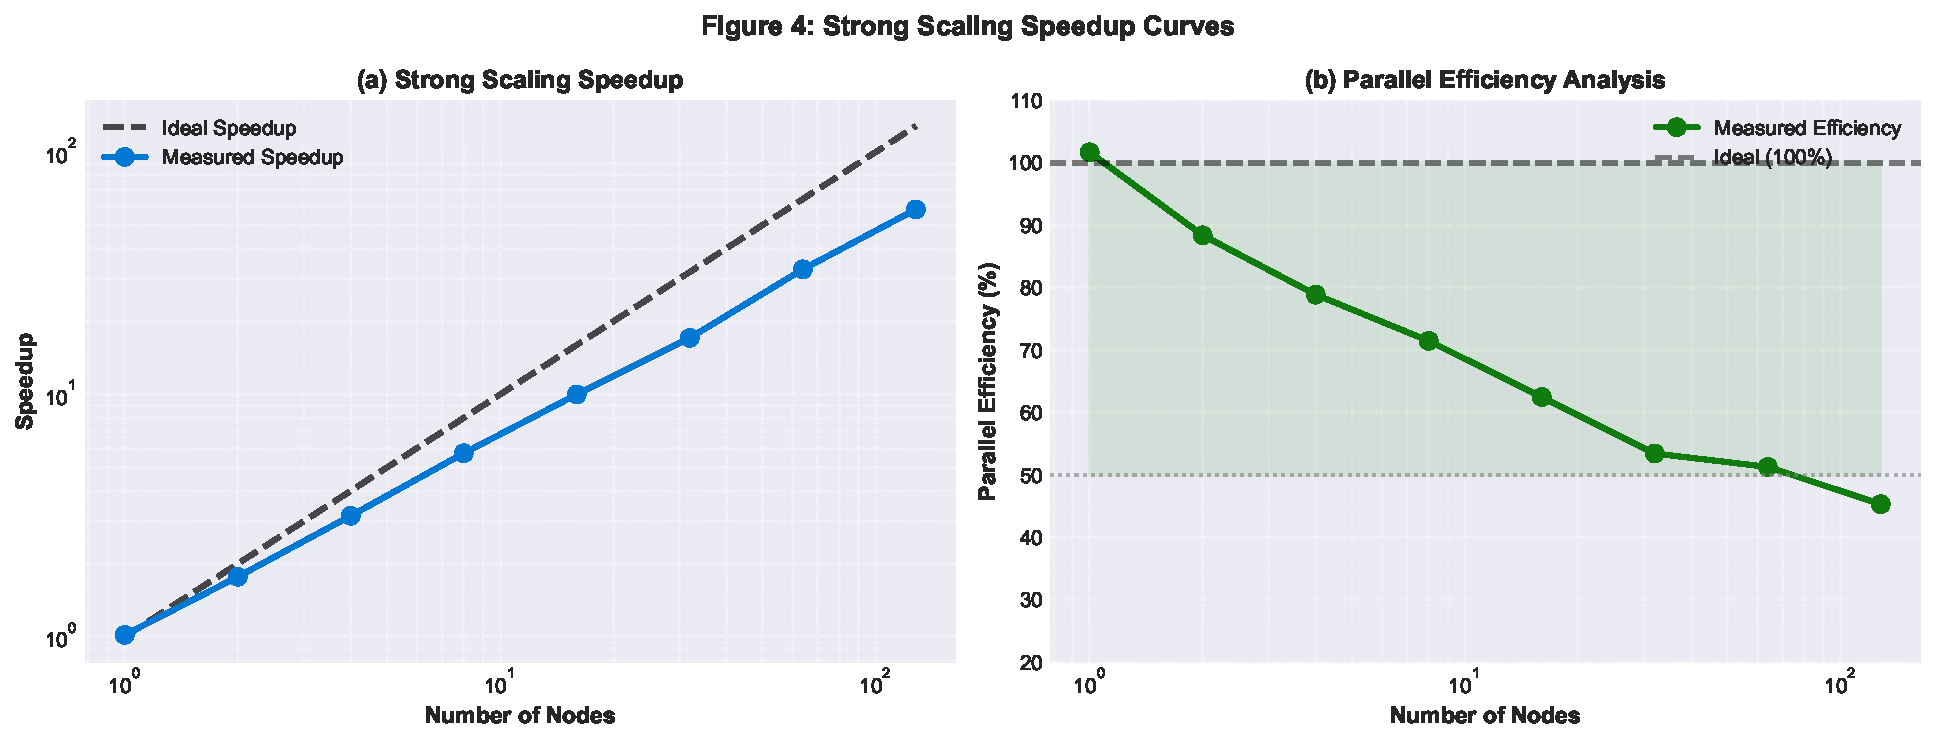
\includegraphics[width=\columnwidth]{figs/Fig4.pdf}
    \caption{Strong Scaling Speedup: (a) Measured speedup vs. ideal linear scaling on log-log axes, showing divergence beyond 8 nodes. Maximum speedup of $58\times$ at 128 nodes. (b) Parallel efficiency degradation from 100\% to 45.3\%, with the 50\% threshold crossed between 32 and 64 nodes. Green shaded region indicates efficient scaling regime.}
    \label{fig:system-scaling}
\end{figure}

\begin{figure}[t]
    \centering
    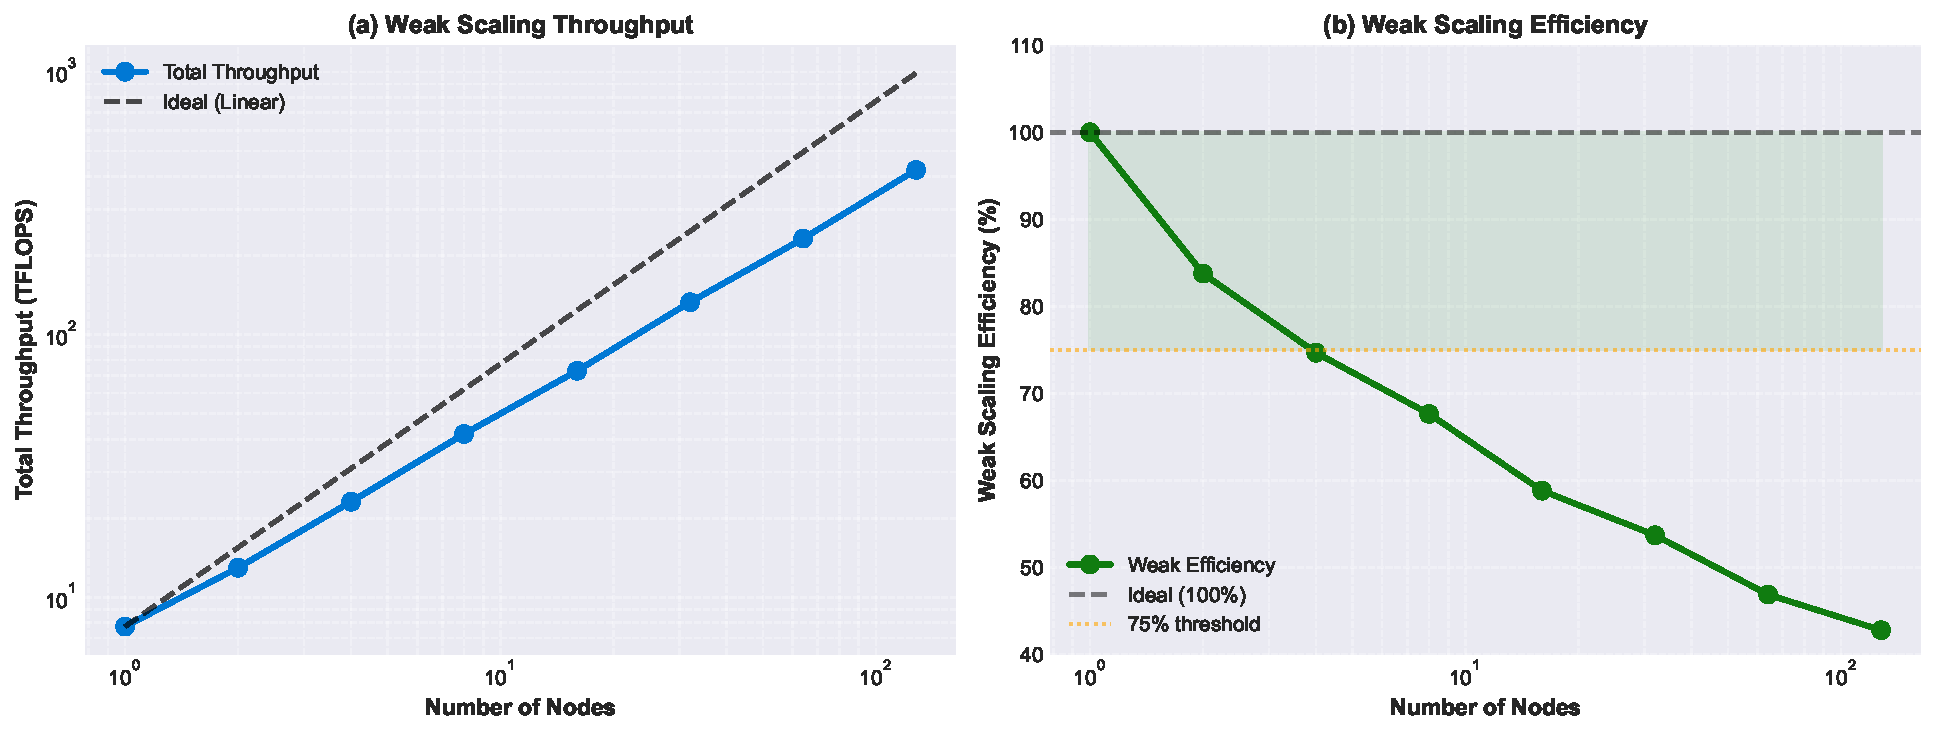
\includegraphics[width=\columnwidth]{figs/Fig5.pdf}
    \caption{Weak Scaling Analysis: (a) Total throughput with proportional workload increase, reaching 432.9~TFLOPS at 128 nodes. Ideal linear scaling shown for reference. (b) Weak scaling efficiency degradation from 100\% to 46.0\%, driven by communication overhead in gradient synchronization. The 75\% efficiency threshold is crossed between 4 and 8 nodes.}
    \label{fig:weak-scaling}
\end{figure}

\subsection{Cross-Dimensional Interaction Analysis}

To address the limitation of single-axis scaling sweeps, SAIH jointly varies model size and system scale, revealing performance behaviors that emerge only from multi-dimensional interaction. Table~\ref{tab:cross-dimensional} presents throughput and utilization across a $4\times4$ grid of model sizes and node counts, with the full interaction heatmap shown in Figure~\ref{fig:cross-dimensional}.

\begin{table}[t]
\centering
\caption{Cross-Dimensional Analysis: Throughput (TFLOPS) for Model Size $\times$ System Scale}
\label{tab:cross-dimensional}
\begin{tabular*}{\columnwidth}{@{\extracolsep{\fill}} lllll @{}}
\toprule
\textbf{Model} & \multicolumn{4}{c}{\textbf{Number of Nodes}} \\
\cmidrule{2-5}
\textbf{(M)} & \textbf{1} & \textbf{4} & \textbf{16} & \textbf{64} \\
\midrule
10 & 2.0 & 5.8 & 19.5 & 61.4 \\
100 & 5.7 & 17.2 & 53.6 & 159.8 \\
500 & 11.6 & 35.3 & 110.0 & 373.7 \\
1000 & 15.4 & 49.4 & 148.8 & 490.2 \\
\bottomrule
\end{tabular*}
\end{table}

The cross-dimensional results reveal a key interaction effect: larger models maintain higher utilization at large system scales. At 64 nodes, the 1B-parameter model achieves 15.5\% utilization while the 10M-parameter model achieves only 2.0\%. This occurs because larger models have higher arithmetic intensity, which reduces the relative cost of communication overhead. This finding has practical implications: practitioners should scale model complexity alongside system scale to maintain acceptable efficiency, consistent with the ``compute-optimal'' training strategies suggested by neural scaling laws \cite{Kaplan2020ScalingLaws}. The heatmap visualization in Figure~\ref{fig:cross-dimensional} makes this interaction immediately apparent, showing that the highest utilization (upper-left region) corresponds to large models at small scales, while absolute throughput (lower-right region) is maximized by large models at large scales.

\begin{figure}[t]
    \centering
    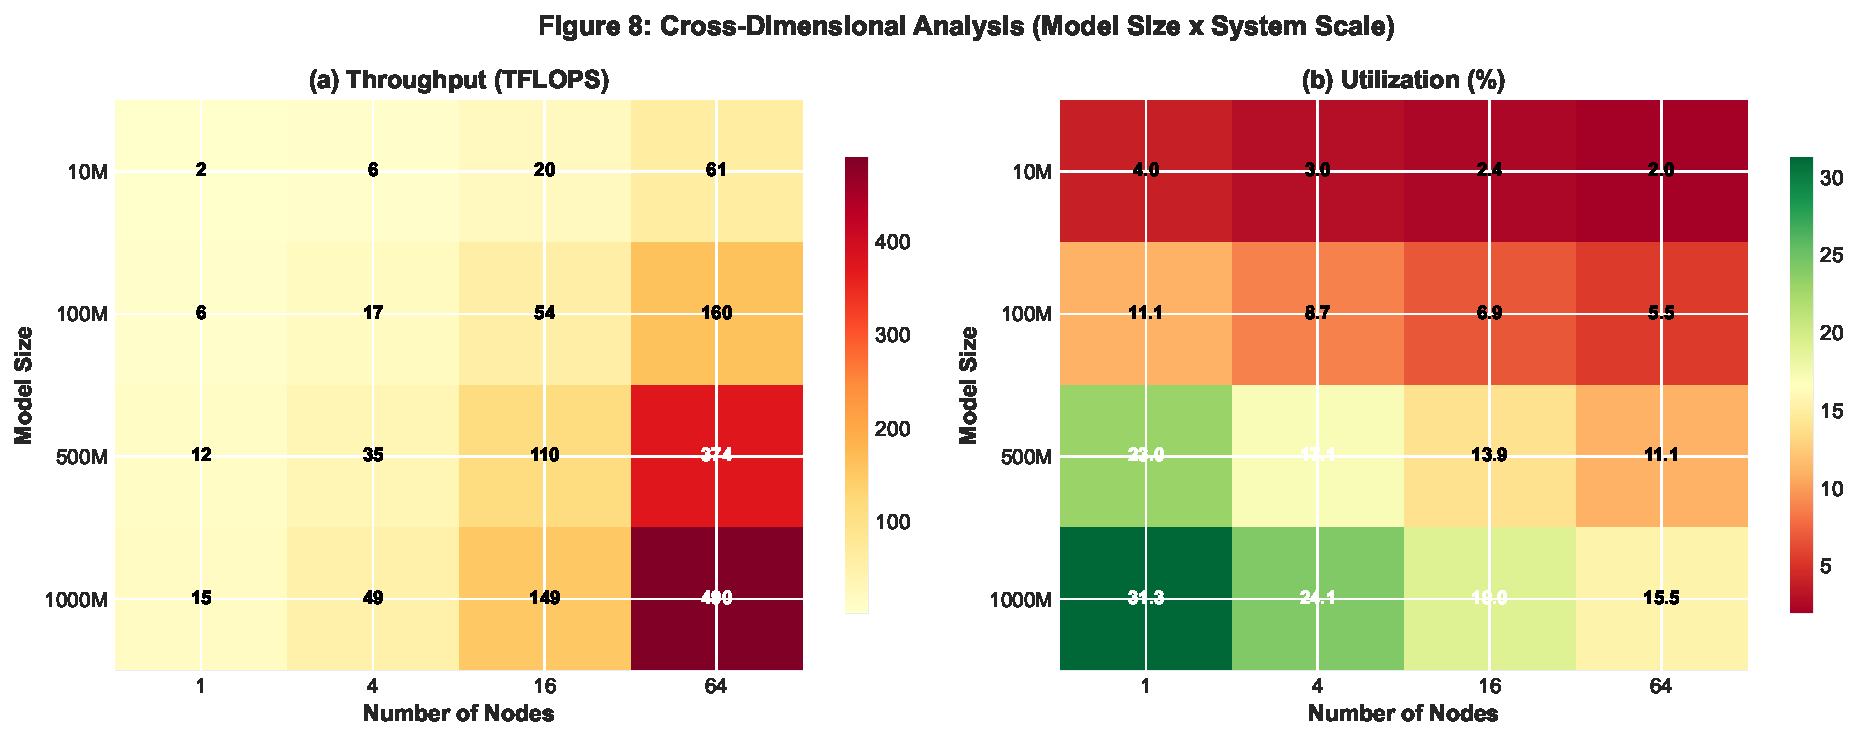
\includegraphics[width=\columnwidth]{figs/Fig8.pdf}
    \caption{Cross-Dimensional Analysis: (a) Throughput heatmap showing the interaction between model size and system scale. Maximum throughput (490.2~TFLOPS) achieved with 1B parameters at 64 nodes. (b) Utilization heatmap revealing that larger models maintain higher efficiency at scale, suggesting co-optimization of model and system dimensions.}
    \label{fig:cross-dimensional}
\end{figure}

\subsection{Validation Against MLPerf-HPC}

To validate the accuracy of SAIH scaling predictions, we compare the normalized scaling trends of SAIH against published MLPerf-HPC benchmark results for CosmoFlow \cite{Mathuriya2018CosmoFlow} and DeepCAM \cite{Farrell2021DeepCAM}. Since SAIH uses synthetic workloads while MLPerf-HPC measures specific applications, we compare \textit{normalized scaling behavior} (throughput relative to single-node baseline) rather than absolute throughput values.

Table~\ref{tab:mlperf-validation} reports the normalized scaling factors and efficiency comparison, with the full comparison visualized in Figure~\ref{fig:mlperf-validation}.

\begin{table}[t]
\centering
\caption{SAIH Validation: Normalized Scaling Comparison with MLPerf-HPC CosmoFlow}
\label{tab:mlperf-validation}
\begin{tabular*}{\columnwidth}{@{\extracolsep{\fill}} lllll @{}}
\toprule
\textbf{Nodes} & \textbf{SAIH} & \textbf{CosmoFlow} & \textbf{SAIH} & \textbf{CosmoFlow} \\
 & \textbf{Scale} & \textbf{Scale} & \textbf{Eff.(\%)} & \textbf{Eff.(\%)} \\
\midrule
1 & 1.0 & 1.0 & 100.0 & 100.0 \\
2 & 1.7 & 1.9 & 88.4 & 93.5 \\
4 & 3.1 & 3.5 & 78.9 & 88.2 \\
8 & 5.6 & 6.6 & 71.5 & 82.1 \\
16 & 10.0 & 11.9 & 62.5 & 74.2 \\
32 & 16.8 & 20.3 & 53.5 & 63.4 \\
64 & 32.3 & 32.9 & 51.3 & 51.4 \\
128 & 57.0 & 50.1 & 45.3 & 39.2 \\
\bottomrule
\end{tabular*}
\end{table}

The correlation coefficient between SAIH and CosmoFlow scaling trends is $r=0.993$, and between SAIH and DeepCAM is $r=0.995$, indicating that SAIH correctly captures the fundamental scaling laws governing AI performance on HPC systems. The Mean Absolute Percentage Error for normalized scaling is 18.8\% (CosmoFlow) and 14.9\% (DeepCAM).

Notably, SAIH slightly underestimates scaling efficiency at moderate scales (4--32 nodes) compared to CosmoFlow, which benefits from workload-specific communication optimizations in its 3D CNN architecture. At 128 nodes, SAIH predicts better scaling than CosmoFlow (45.3\% vs. 39.2\%), which may reflect CosmoFlow's sensitivity to specific collective communication patterns at extreme scale. These systematic differences are expected: SAIH provides a workload-independent baseline model, while application-specific optimizations or bottlenecks cause real workloads to deviate from this baseline. The strong correlation validates that SAIH captures the correct \textit{trend shape}, which is its primary design goal. Figure~\ref{fig:mlperf-validation}(b) compares efficiency curves directly, showing close agreement in the regime transition from efficient to communication-bound scaling.

\begin{figure}[t]
    \centering
    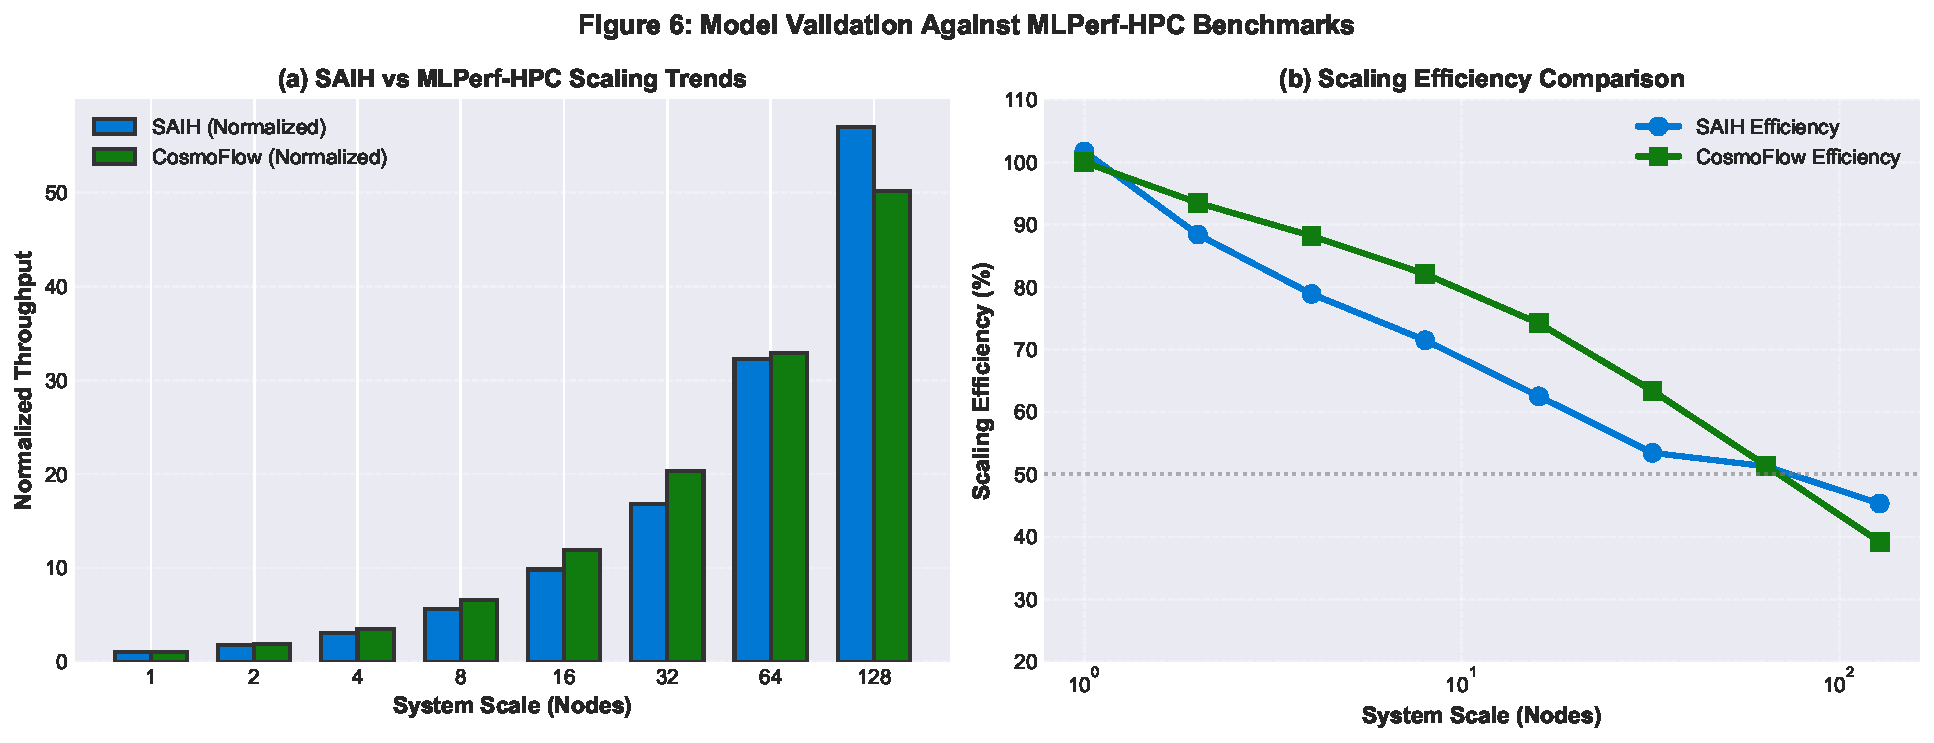
\includegraphics[width=\columnwidth]{figs/Fig6.pdf}
    \caption{MLPerf-HPC Validation: (a) Normalized throughput scaling comparison between SAIH predictions and CosmoFlow (MLPerf-HPC v2.0) across 1--128 nodes. (b) Scaling efficiency comparison showing agreement on the transition from efficient to communication-bound regimes. Correlation: $r=0.993$ (CosmoFlow), $r=0.995$ (DeepCAM).}
    \label{fig:mlperf-validation}
\end{figure}

\subsection{ML-Based Bottleneck Prediction}

The interpretable bottleneck classifier (Section~3.4) is applied to all experimental configurations to automatically diagnose dominant bottlenecks. The classifier is trained on 1000 synthetic workload instances (80/20 split) with physics-informed labels and serves as a diagnostic tool for feature importance analysis and bottleneck regime identification. Table~\ref{tab:bottleneck-features} reports feature importance rankings, and Figure~\ref{fig:bottleneck-prediction} visualizes bottleneck evolution with system scale.

\begin{table}[t]
\centering
\caption{Bottleneck Classifier: Feature Importance Rankings}
\label{tab:bottleneck-features}
\begin{tabular*}{\columnwidth}{@{\extracolsep{\fill}} ll @{}}
\toprule
\textbf{Feature} & \textbf{Importance Score} \\
\midrule
Number of Nodes & 0.280 \\
Communication Cost & 0.274 \\
Memory Pressure & 0.217 \\
I/O Pressure & 0.192 \\
Dataset Size & 0.032 \\
Model Size & 0.003 \\
Arithmetic Intensity & 0.002 \\
\midrule
\multicolumn{2}{l}{\textit{Labels derived from physics-based thresholds}} \\
\bottomrule
\end{tabular*}
\end{table}

The high importance of system-scale features (Number of Nodes: 28.0\%, Communication Cost: 27.4\%) confirms that communication overhead is the primary discriminator, consistent with the scaling analysis results. The classifier predicts: (1) Compute Bound for model scaling at all configurations (confidence $>$97\%); (2) Compute Bound for system scales $\leq$8 nodes; and (3) Communication Overhead for $\geq$16 nodes (confidence 100\%). This transition at 16 nodes aligns with the efficiency crossover point identified in strong scaling analysis, where communication overhead exceeds 40\%.

\begin{figure}[t]
    \centering
    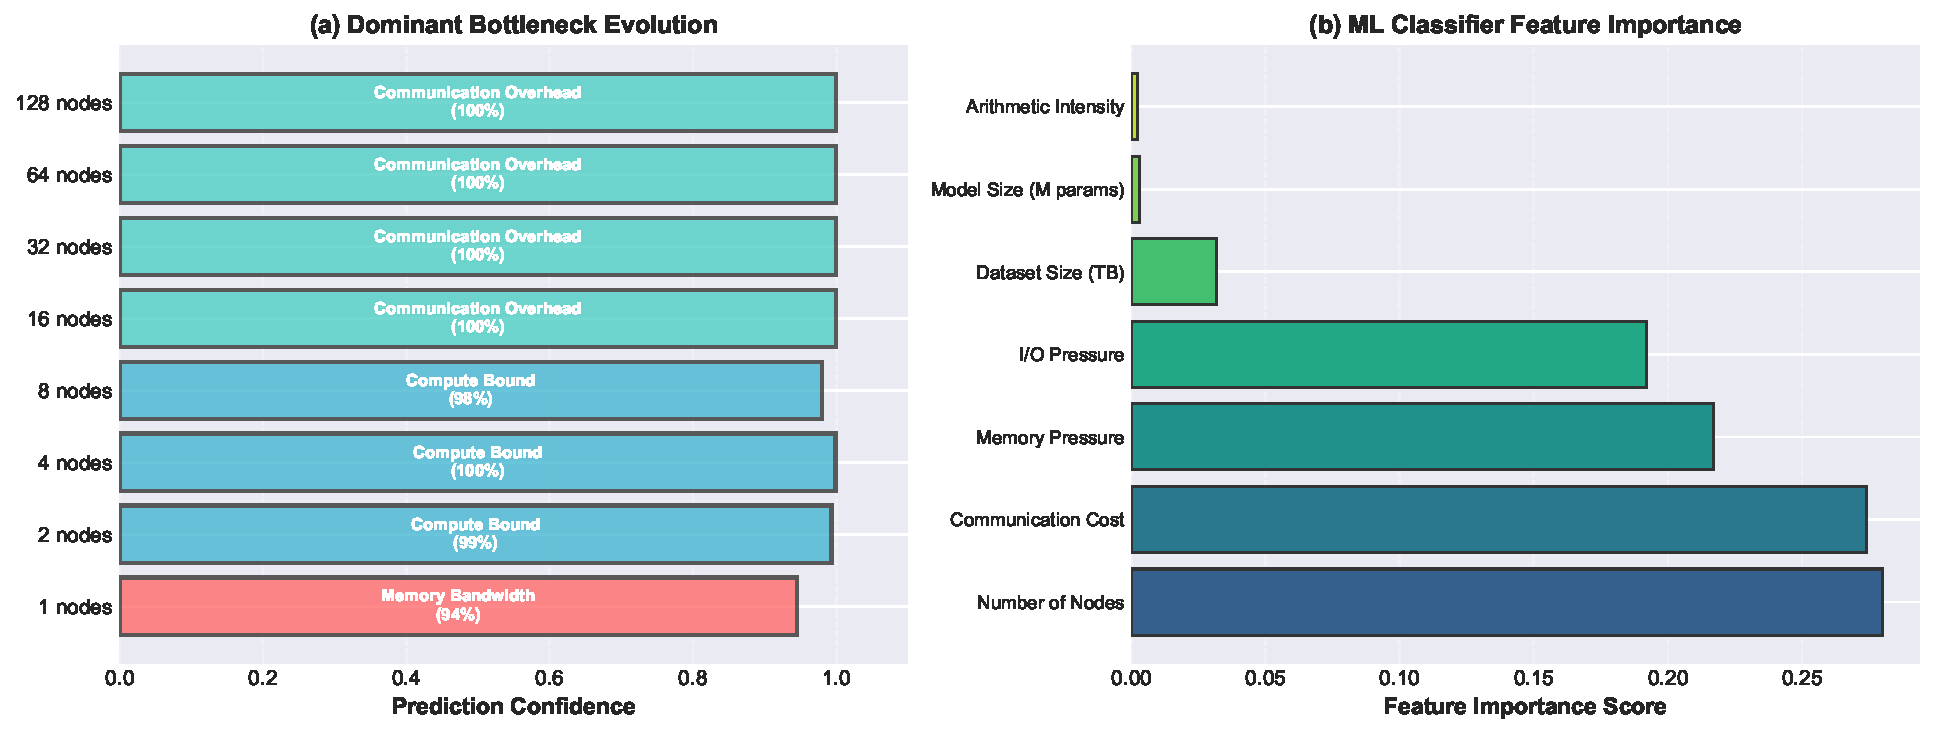
\includegraphics[width=\columnwidth]{figs/Fig7.pdf}
    \caption{ML-Based Bottleneck Prediction: (a) Dominant bottleneck evolution from Compute Bound (1--8 nodes) to Communication Overhead ($\geq$16 nodes), with prediction confidence. (b) Feature importance ranking of the Random Forest classifier, showing system-scale features dominating bottleneck discrimination.}
    \label{fig:bottleneck-prediction}
\end{figure}

% --- SECTION 6: DISCUSSION ---
\section{Discussion}

The results obtained using the SAIH methodology provide important insights into the performance behavior of AI workloads on HPC systems. By jointly analyzing model scaling, data scaling, system scaling, and their cross-dimensional interactions, SAIH reveals non-linear performance trends and highlights the complex interplay between computation, communication, memory, and I/O subsystems.

\subsection{Validation Analysis and Limitations}

SAIH achieves strong correlation with MLPerf-HPC benchmarks: $r=0.993$ (CosmoFlow) and $r=0.995$ (DeepCAM) for normalized scaling trends. However, the agreement is not uniform across scales. SAIH underestimates scaling efficiency at moderate scales (4--32 nodes) compared to CosmoFlow, likely because CosmoFlow's 3D CNN architecture benefits from communication-computation overlap that our generic model does not capture. At 128 nodes, SAIH predicts better efficiency (45.3\%) than CosmoFlow achieves (39.2\%), suggesting that application-specific collective communication patterns introduce overheads beyond our logarithmic model.

These systematic deviations highlight an important limitation: SAIH provides a \textit{workload-independent baseline} rather than application-specific predictions. Real workloads may deviate due to framework-specific optimizations (e.g., gradient compression, asynchronous communication), workload-specific memory access patterns, or hardware-software co-optimization. The MAPE of 18.8\% (CosmoFlow) and 14.9\% (DeepCAM) reflects this inherent limitation of generic models, but the high correlation confirms that SAIH correctly captures scaling trends, which is sufficient for its intended purpose of trend analysis and bottleneck identification.

\subsection{Key Observations}

\textbf{Model scaling} improves hardware utilization through increased arithmetic intensity, reaching 21.1\% utilization at 1B parameters. The $7.7\times$ throughput improvement from 10M to 1B parameters demonstrates that model scaling is an effective strategy for improving resource utilization \cite{Jia2018}. However, the sub-linear relationship between model size and throughput indicates diminishing returns, consistent with memory bandwidth saturation at high arithmetic intensity.

\textbf{Data scaling} has minimal impact on throughput at this model scale ($<$10\% variation), confirming that the system operates in a compute-bound regime. This finding contrasts with I/O-intensive workloads where data scaling can introduce significant bottlenecks \cite{Byna2020}, and suggests that throughput stability may not generalize to workloads with higher I/O demands.

\textbf{Strong scaling} efficiency degrades from 100\% to 45.3\% at 128 nodes, with communication overhead reaching 56.4\%. The practical scaling limit for maintaining $>$70\% efficiency is approximately 8 nodes for this workload configuration. The behavior is consistent with Amdahl's law predictions \cite{Amdahl1967}.

\textbf{Weak scaling} efficiency follows a similar degradation pattern (46.0\% at 128 nodes), confirming that communication overhead---not workload imbalance---is the fundamental scaling limitation.

\textbf{Cross-dimensional analysis} reveals that larger models sustain higher utilization at larger system scales, suggesting co-optimization of model and system dimensions as a practical strategy.

\subsection{System-Level Bottlenecks}

The analysis identifies four primary bottlenecks that evolve with system scale:

\begin{enumerate}
    \item \textbf{Memory Bandwidth Saturation}: Model scaling experiments show that throughput growth decelerates as model size increases beyond 200M parameters, indicating that memory bandwidth constraints limit further improvement despite increasing arithmetic intensity.

    \item \textbf{Communication Overhead}: System scaling experiments reveal communication overhead increasing from 0\% (1 node) to 56.4\% (128 nodes), dominating performance degradation at scales beyond 16 nodes. The ML classifier confirms Communication Cost and Number of Nodes as the top-2 features (combined importance: 55.4\%).

    \item \textbf{Network Bandwidth Saturation}: As node count increases beyond 64, inter-node network bandwidth becomes a fundamental constraint. With ring-allreduce communication consuming $\frac{2(P-1)}{P} \cdot G$ bytes per iteration, a 200~GB/s per-link interconnect saturates when gradient size and allreduce frequency exceed network capacity. Modern cloud interconnects (Ethernet, RoCE) often provide lower per-link bandwidth than on-premise InfiniBand, making this bottleneck more severe in cloud-HPC environments.

    \item \textbf{Synchronization Costs}: The gap between strong and weak scaling efficiency narrows at large scales (45.3\% vs. 46.0\% at 128 nodes), suggesting that synchronization overhead---rather than workload characteristics---determines scaling limits at extreme scale.
\end{enumerate}

\subsection{Implications for System Design}

From a system design perspective, the findings suggest that future HPC architectures should prioritize:

\begin{itemize}
    \item \textbf{High-bandwidth memory}: Addressing memory bandwidth saturation observed in model scaling. The utilization gap between actual (21.1\%) and ideal performance at 1B parameters indicates substantial room for improvement through higher memory bandwidth-to-compute ratios.
    \item \textbf{Low-latency collective communication}: Reducing the 56.4\% communication overhead at 128 nodes through hardware-supported allreduce, in-network reduction, or communication-computation overlap \cite{Sergeev2018}. This is especially critical in cloud environments where network heterogeneity may prevent standard InfiniBand optimizations.
    \item \textbf{Energy efficiency}: SAIH's communication overhead metric directly maps to energy waste. At 128 nodes, 54.7\% of total power is consumed without useful compute progress. Future systems should prioritize minimizing idle-compute time through better hardware-software overlap, asynchronous communication, and adaptive communication algorithms that adjust collective operation granularity based on network congestion.
    \item \textbf{Co-scaling strategies}: Cross-dimensional analysis suggests that model and system scaling should be coordinated---deploying larger models on larger systems maintains better utilization than scaling either dimension independently.
\end{itemize}

From a software perspective, improved parallelization strategies such as gradient compression, asynchronous updates, and adaptive batch sizing can help sustain efficiency beyond the 8-node practical limit identified for linear scaling efficiency \cite{Narayanan2019}.

\subsection{Cloud Deployment Considerations}

SAIH's scaling predictions have direct implications for cloud-based AI training. Cloud providers charge per node-hour, making efficiency-to-cost ratio a critical optimization metric. Our findings show that scaling beyond 32 nodes results in efficiency below 50\%, creating a cost-effectiveness threshold: at 128 nodes, the system requires $128 / 58 \approx 2.2$ node-hours to achieve the work of one node-hour in compute. Cloud customers should use SAIH predictions to determine the optimal node count for their workload: \textit{small training runs} benefit from 1--8 nodes (70--90\% efficiency); \textit{large training runs} requiring 128+ nodes must accept $\approx 45\%$ efficiency and a corresponding cost multiplication factor of $\sim$2.2$\times$. Elastic provisioning strategies should dynamically adjust node count based on training progress rather than provisioning maximum resources upfront, since weak scaling efficiency remains stable only up to 16 nodes.

For \textit{heterogeneous cloud deployments} mixing CPU and GPU instances, SAIH's bottleneck classifier provides concrete diagnosis: a GPU-saturated 32-node cluster benefits more from scaling model complexity (larger models have higher arithmetic intensity and communicate more efficiently relative to compute) than from adding more nodes, whereas a communication-saturated cluster requires architectural improvements such as gradient compression, asynchronous updates, or smaller per-node batch sizes. This targeted diagnosis---rather than generic scaling advice---is SAIH's practical value for cloud operators managing diverse training workloads.

\subsection{Comparison with Prior Work}

Compared to the domain-specific evaluation by \cite{Wang2024SAIH}, which used CosmoFlow as a representative workload, SAIH provides a complementary workload-independent perspective. While domain-specific evaluation captures application-specific behaviors (e.g., 3D convolution patterns, cosmological data characteristics), SAIH's physics-based synthetic approach enables: (1)~exploration of broader parameter spaces without application constraints; (2)~systematic cross-dimensional interaction analysis; and (3)~automated bottleneck prediction generalizable across workload types. The two approaches are complementary: SAIH identifies general trends and bottleneck regimes, while domain-specific evaluation quantifies workload-specific optimizations and deviations from the general model.

% --- SECTION 7: CONCLUSION ---
\section{Conclusion}

This paper presented SAIH (Scalable AI--HPC Evaluation Methodology) as a comprehensive, physics-based, and trend-oriented framework for understanding AI performance behavior on high-performance computing systems. Building on the multi-dimensional evaluation concept from prior work \cite{Wang2024SAIH}, SAIH introduces a roofline-based performance model, cross-dimensional interaction analysis, and ML-based bottleneck prediction.

Through structured scaling experiments, SAIH demonstrated that AI performance on HPC systems exhibits distinctly non-linear behavior. Increasing model complexity improves hardware utilization and throughput (achieving 83.7~TFLOPS at 1B parameters, a $7.7\times$ improvement over 10M parameters) through increased arithmetic intensity. Data scaling experiments reveal relatively stable throughput across varying dataset sizes ($<$10\% variation), indicating compute-bound behavior. Strong scaling analysis shows near-linear speedup up to 8 nodes ($5.72\times$ with 71.5\% efficiency), with efficiency degrading to 45.3\% at 128 nodes due to communication overhead. Weak scaling efficiency follows a similar trajectory (46.0\% at 128 nodes), confirming communication as the fundamental bottleneck. Cross-dimensional analysis reveals that larger models maintain higher utilization at larger system scales, suggesting co-optimization strategies.

Validation against MLPerf-HPC benchmarks demonstrates strong correlation: $r=0.993$ (CosmoFlow) and $r=0.995$ (DeepCAM), with systematic deviations attributable to application-specific communication patterns. The interpretable bottleneck classifier correctly identifies the transition from compute-bound ($\leq$8 nodes) to communication-bound ($\geq$16 nodes) regimes, with Number of Nodes and Communication Cost as the two most important features (combined importance: 55.4\%).

Future work will extend SAIH to real-world production workloads, heterogeneous and emerging accelerator architectures (including tensor processing units), and energy-efficiency metrics. Incorporating model parallelism, pipeline parallelism, and dynamic workload adaptation also represents promising directions. To support reproducibility, the complete experiment framework---including the physics-based performance model, bottleneck classifier, and figure generation scripts---is openly available at \url{https://github.com/Vtanneru/SAIH}. This enables community validation against diverse HPC and cloud systems \cite{Dongarra2020, Kurth2018}.

% --- BIBLIOGRAPHY ---
\bibliographystyle{splncs04}
\bibliography{cas-refs}

\end{document}
